\chapter{Indledning}

\noindent Når man bor i et bofællesskab, er der mange bolde der skal holdes i luften. Udover man eventuelt har eget værelse, er der også et fælles ansvar for bofællesskabet der gælder for flere områder. Hvem skal rengøre huset, og hvornår skal det gøres? Hvem har vaskemaskinen i dag? Er der en fælles madplan, og hvem er med i den? Kommer familien på besøg, eller er der fest i weekenden og mange andre ting der internt skal koordineres. \\ \textbf{Indsæt reference om at verbale aftaler kan være svære at koordinere og overholde} Det er svært at koordinere med hinanden verbalt, da folk har travlt med deres hverdag, hurtigt glemmer beskeder og måske ikke ender med at få en besked ud til alle personer. På baggrund af dette har projektet til formål at optimere håndteringen af de ovenstående temaer.

%\noindent I dette projekt er der derfor blevet gjort fokus på at lave en webapplikation til bofællesskaber, som vil være et centralt sted til at kommunikere, planlægge og strukturere dagligdagen for bofællesskabet. Dette projekt bliver kaldt for WePlanner.

\section{Problemformulering}
Med udgangpunkt i projektets formål er der i gruppen kommet frem til følgende problemformulering:
\begin{center}

\textit{"Hvordan kan man via en webapplikation løse planlægningsmæssige}\\
\textit{problematikker i bofællesskaber og andre sociale sammenhænge?}
\vspace{5mm}\\\textbf{Not so good:}
\textit{''Hvordan kan man løse problemet vha. en webapplikation,}

\textit{og hvad skal applikationen indeholde så den simplificerer overblik''} \\
\end{center}

\noindent Med udgangspunkt i problemformulering, er det ønsket fra projektgruppens side at udvikle produktet \textit{WePlanner}.

\section{Produktbeskrivelse}
\noindent WePlanner er en webapplikation som gør det nemmere for forskellige grupper/fællesskaber, som kollegier, bofællesskaber, fodboldklubber osv., at kunne kommunikere med hinanden. I den første udgave af webapplikationen, er der lagt fokus på at lave et fuldendt kommunikationsværktøj for bofællesskaber og kollegier, og senere hen udvikle det til at kunne bruges af andre grupper og fællesskaber.\\

\noindent En bruger opretter sig på hjemmesiden, og kan nu oprette en gruppe for sit fællesskab, eller blive inviteret til et allerede eksisterende board, via. E-mail. Den bruger der opretter gruppen, er automatisk administratoren af gruppen, og har dermed flere rettigheder end de andre brugere. Flere brugere kan godt blive gjort til administrator af gruppen. \\

\noindent Når gruppen er oprettet, kan administratoren tilføje widgets til dette board, som hver især har forskellige egenskaber. Når man er inde på gruppens forside, vises alle de tilføjede widgets med en overskrift, og en lille meddelelse, med den vigtigste information fra den enkelte widget.\\
På denne måde kan man udefra gruppens forside, få et godt overblik af relevant information. Ved at klikke på en widget, udvides denne og al information kan findes heri.

\noindent De widgets der i første omgang er planlagt er følgende

\begin{itemize}
\item  \textbf{Kalender}

Her kan brugere skrive begivenheder ind, som er relevant for de andre brugere i gruppen.
\end{itemize}

\begin{itemize}
\item  \textbf{Pinned event}

Bruges til at high light'e en begivenhed hvis den er meget vigtig.
\end{itemize}

\begin{itemize}
\item  \textbf{Booking}

Her kan brugere gå ind og booke ressourcer og se hvornår ressourcen er booket. Dette kan f.eks. bruges til at lave et bookingsystem af en fælles vaskemaskine.
\end{itemize}

\begin{itemize}
\item  \textbf{Planlægning}

Denne bruges til at lave planlægning over faste opgaver. Brugere kan så gå ind og se hvornår det er deres tur, og bytte deres vagter med de andre brugere. Dette kan f.eks. bruges til at lave en madplan eller rengøringsplan.
\end{itemize}

\begin{itemize}
\item  \textbf{Liste}

\noindent Kan bruges til at oprette en liste, som brugerende kan tilføje elementer til. Denne kan f.eks. bruges til at lave en fælles indkøbsliste.
\end{itemize}

\begin{itemize}
\item  \textbf{Betaling}

\noindent Her kan en bruger skrive ind hvis han/hun har lagt ud for noget, som nogle af de andre brugere skal betale for. De betalende brugere går ind og markerer når de har betalt, og den betalende bruger accepterer at der er betalt tilbage.
\end{itemize}

\begin{itemize}
\item  \textbf{Opslagstavle}

\noindent Her kan brugere skrive et opslag, der kan være relevant for de andre brugere. Denne widget kan som den eneste deles med andre boards. På den måde kan den fungere som en fælles opslagstavle for en hel opgang, uden at opgangen skal have et fælles board.
\end{itemize}
\noindent Brugeren med rollen \textbf{Administrator} tilføjer selv de widgets der kan have relevans for den gruppe der er oprettet. De forskellige widgets som tilføjes, har hver deres indstillingsmuligheder, så de kan sættes op så de passer til det som brugerende vil bruge dem til. 

\subsection{Visuellisering af produkt}
For at tydeliggøre hvordan ideen visuelt ser ud, er der herunder lavet nogle billeder til at understøtte dette. Herunder på figur \ref{fig:login_site} er login siden vidst. Det er det første man som bruger møder, hvor det her er muligt at logge ind med sin e-mail og password. Derudover er det også muligt at oprette en bruger, selvom dette ikke er vist.
\begin{figure}[H]
  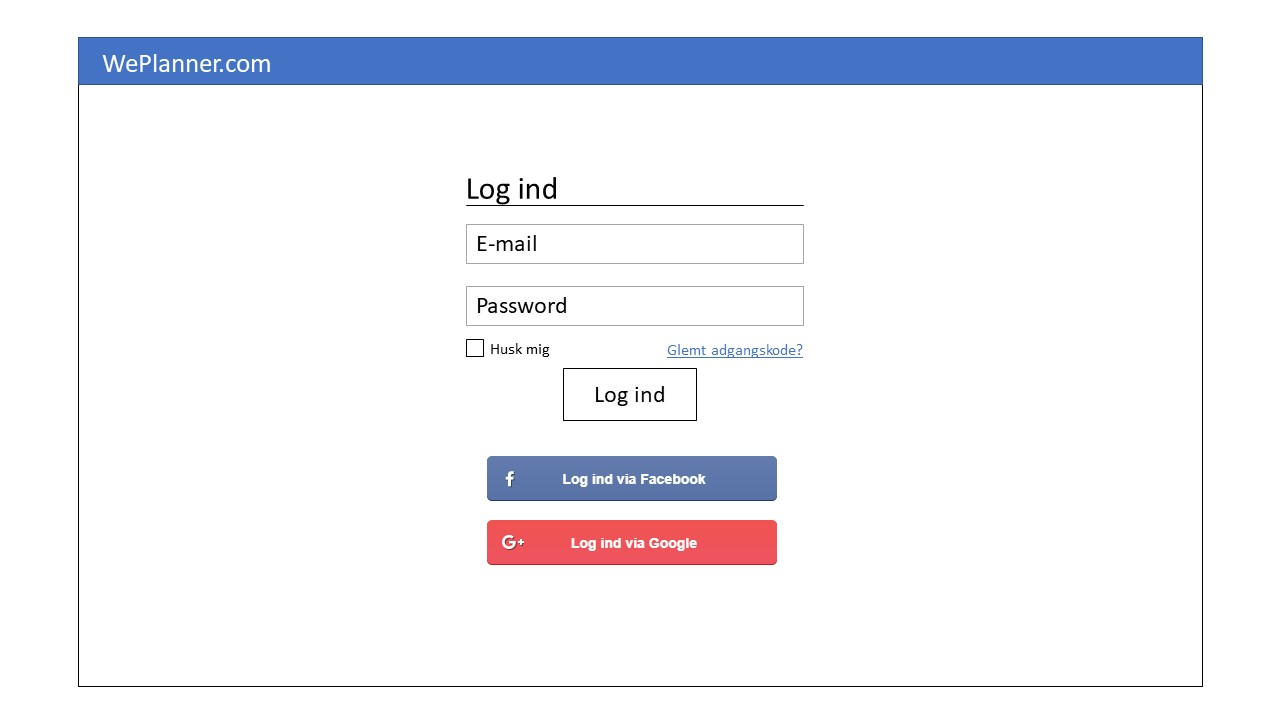
\includegraphics[width=\linewidth]{Indledning/Images/Slide1.JPG}
  \caption{Login side}
  \label{fig:login_site}
\end{figure}

\noindent Når man er logget ind med sin bruger, møder man 'Home' siden, som kan ses på figur \ref{fig:home_site}. Her kan brugeren se alle de boards som brugeren er medlem af. Derudover har brugeren også mulighed for at oprette en gruppe.
\begin{figure}[H]
  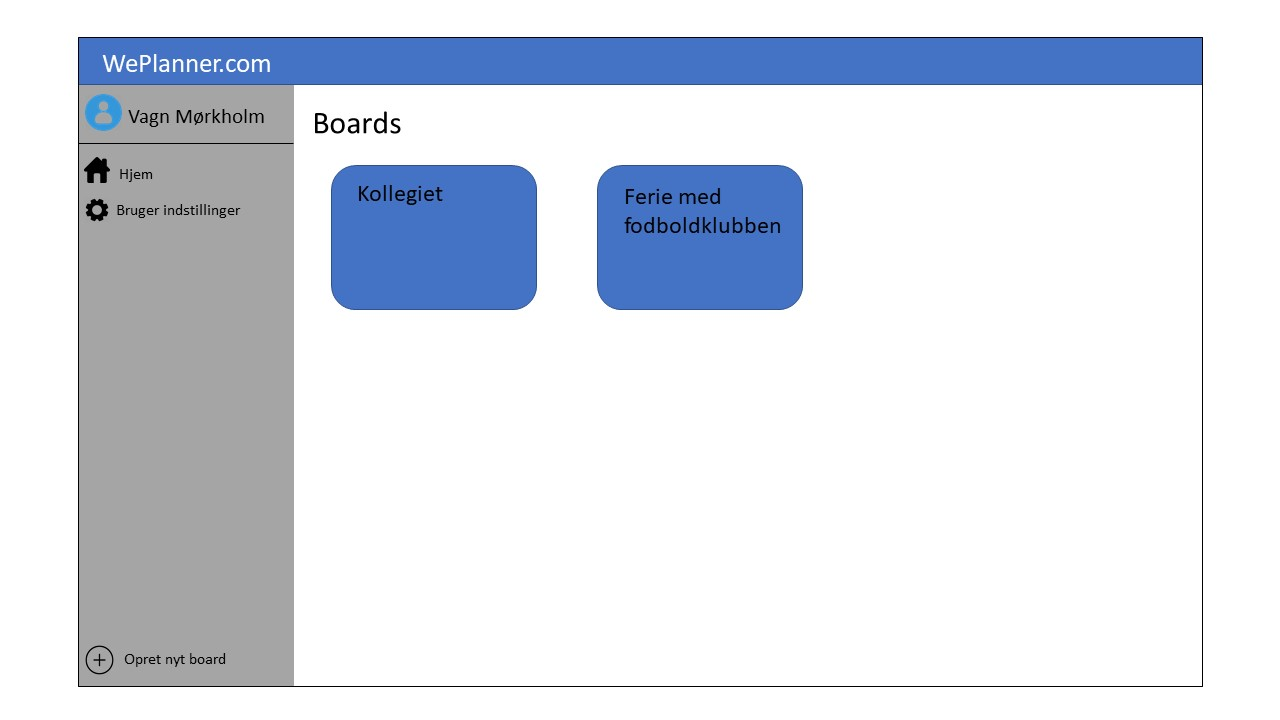
\includegraphics[width=\linewidth]{Indledning/Images/Slide2.JPG}
  \caption{Home side}
  \label{fig:home_site}
\end{figure}

\noindent Ved at vælge en gruppe, kommer man ind på en ny side som viser gruppen med alle de tilføjede widgets. Her kan brugeren få et hurtigt overblik ved at kigge på de forskellige widgets. Brugeren kan så trykke på en widget, som udvider sig og giver flere informationer. Dette ses på figur \ref{fig:board_site}.
\begin{figure}[H]
  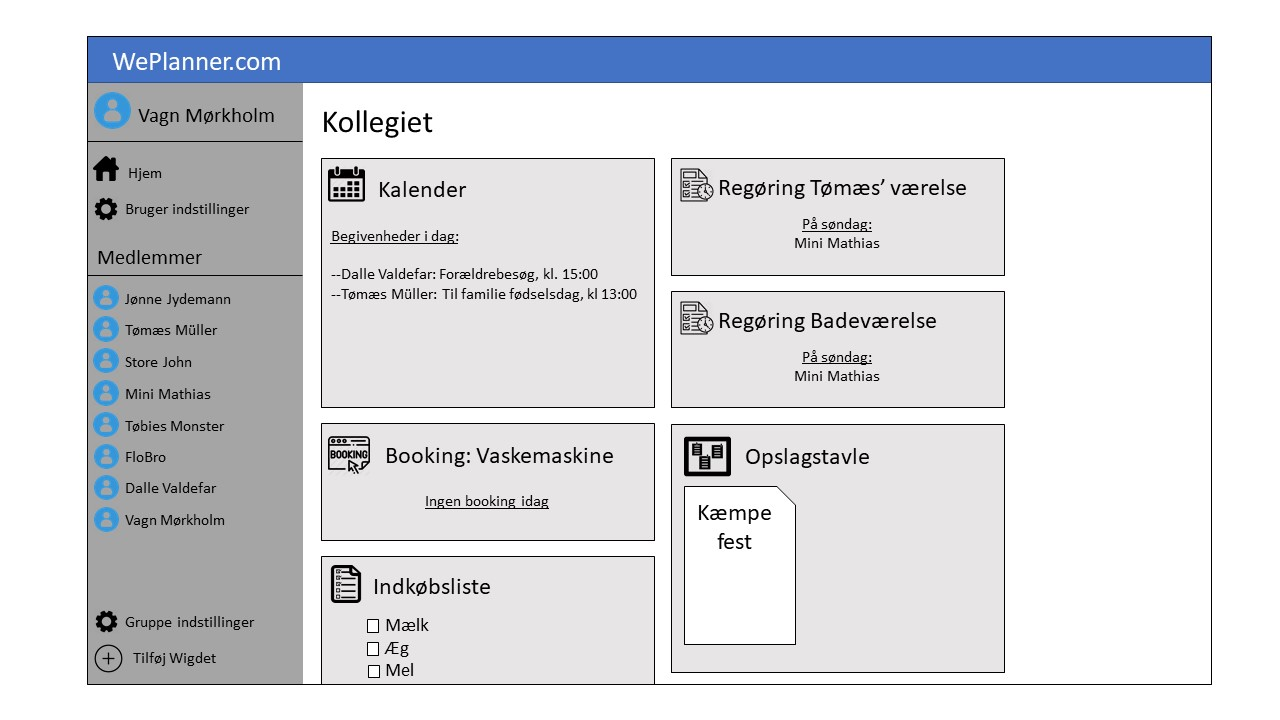
\includegraphics[width=\linewidth]{Indledning/Images/Slide3.JPG}
  \caption{Board side}
  \label{fig:board_site}
\end{figure}

\section{MoSCoW}
Der foretages en MoSCoW analyse for at få et overblik over Applikationens ønskede funktionalitet, samt at prioritere implementeringen af applikationens forskellige elementer. MoSCoW analyse danner således baggrund for udviklingsprocessen.
\newline\newline

\noindent \textbf{Must have:}

\begin{itemize}
    \item Applikationen skal have en login-funktion og mulighed for at oprette brugere
    \item En bruger skal identificeres ved e-mail som anvendes ved login
    \item I applikationen skal det være muligt at oprette en gruppe med et default layout, hvortil der kan inviteres medlemmer
    \item Applikationen skal indeholde en kalender
    \item Applikationen skal indeholde funktionalitet der gør det muligt at se og planlægge en madplan og rengøringsplan
    \item Det skal være muligt at bytte rengørings- og mad- vagter mellem brugere. 
    \item Gruppens aktiviteter skal vises på gruppens kalender
    \item Applikationen skal indeholde en opslagstavle for en gruppe.
    \item Web-applikationen skal kommunikere med en server ved brug af en TCP? Forbindelse.
    \item Applikationen skal indeholde en liste widget.
    \item Det skal være muligt for gruppens medlemmer at tilføje og slette forskellige widgets på gruppens side.
    \item Applikationen skal gøre det muligt at oprette et booking system til booking af ressourcer
    \item Applikationen skal have en regnskabs widget.
\end{itemize}

\noindent \textbf{Should have:}

\begin{itemize}
    \item Mulighed for at tilpasse udseendet af boardet
    \item Administrator rettigheder
\end{itemize}

\noindent \textbf{Could have:}

\begin{itemize}
    \item Mulighed for at indsame brugerstatistikker
    \item Integrering med dansk supermarked der udbyder levering af varer
\end{itemize}

\noindent \textbf{Won't have (this time)}
\begin{itemize}
    \item En tilsvarende App til iOS/Android
    \item Integrering med mobilePay/ weshare mm.
\end{itemize}



\section{Udviklingsværktøjer}
